\documentclass[10pt,a4paper,oneside]{book}

\usepackage[slovene]{babel}
\usepackage[utf8x]{inputenc}
\usepackage{makeidx}
\usepackage{graphicx}
\usepackage{enumerate}
\usepackage[margin=1in]{geometry}
\usepackage{verbatim}
\usepackage[svgnames]{xcolor}
\usepackage{fancybox}
\usepackage{varwidth}
\newcommand\inline[1]{%
\begin{Sbox}{#1}\end{Sbox}%
\colorbox{lightgray}{\TheSbox}%
}
\newcommand\inliney[1]{%
\begin{Sbox}\begin{varwidth}{0.91\textwidth}{#1}\end{varwidth}\end{Sbox}%
\colorbox{lightgray}{\TheSbox}%
}

\newcommand\pic[2]{%
\parbox{1cm}{%
\begin{center}%
\includegraphics[width=#1\textwidth]{#2}%
\end{center}%
}%
}

\newcommand\br{%
 \ \\ \ \\%
}

\usepackage{hyperref}
\hypersetup{
    colorlinks=true,
    linkcolor=black,
    urlcolor=blue,
    pdftitle={AngryPigs}
}
\title{AngryPigs}

\begin{document}
\begin{titlepage}
\begin{center}
\ \\[3.5cm]
{\resizebox{16.8cm}{!}{\Huge\bf\color{LightGreen}\texttt{AngryPigs{\tiny\ }}}}\\[-2.8cm]
{\resizebox{16.8cm}{!}{\Huge\bf\color{Green}\texttt{{\tiny\ }AngryPigs}}}\\[3.9cm]
{\Huge\bf Dokumentacija}\\[0.35cm]
{\huge\today}\ \\[4.5cm]
{\Huge {\bf Avtorja}}\\[0.35cm]
{\huge Matic Potočnik, Jaka Sivec}
\vfill
\end{center}
\end{titlepage}
\chapter{O igri}
AngryPigs je zabavna 3D igra, v kateri igralec katapultira prašiče v drevesa, ter skuša z njih sklatiti ptice, ter njihova gnezda. Igra je bila ustvarjena v sklopu seminarske naloge za predmet Računalniška grafika na univerzitetnem programu Fakultete za računalništvo in informatiko v Ljubljani. Repozitorij z izvorno kodo je na voljo na: \inline{\url{https://github.com/HairyFotr/AngryPigs}}
\br
\begin{center}
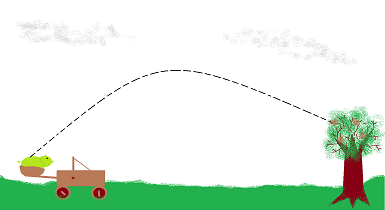
\includegraphics[width=12cm]{conceptsmall}
\end{center}

\chapter{Tehnologija}
\section{Uvod}
Igra je napisana v Scali, z izjemo dela, ki generira drevesa -- ta je bil napisan v jeziku Clojure. Scala je razmeroma nov jezik, ki teče na JVM(Java Virtual Machine) in hkrati podpira objektno ter funkcijsko programiranje. Clojure je moderen dialekt Lispa, ki tudi teče na JVM. Oba sva bila pred začetkom projekta skoraj čista začetnika v obeh jezikih.\\[-7pt]

Za grafiko sva uporabila knjižnico LWJGL. Prevedla in priredila sva nekatere primere iz vaj. Igra ne uporablja naprednih tehnik in funkcionalnosti OpenGL-a, predvsem zato, ker ima Matic precej počasen prenosnik in za nameček na njem poganja Linux, ki ne podpira njegove vgrajene grafične kartice. Grafika mu teče v programsko-pospešenem načinu. (To ni le šala, ampak precej velik faktor pri nekaterih odločitvah)

\section{Prevajanje}
Prvi problem na katerega sva naletela je, kako hkrati prevajati Scalo in Clojure, ter kako v Scali uporabiti funkcije iz Clojura. Oba jezika sta v precejšnji meri kompatibilna z Javo, v smislu, da lahko uporabljata vse Javine razrede, z nekaj truda gre tudi obratno, z še nekaj več truda, pa lahko sodelujeta tudi Scala in Clojure.\\[-7pt]

Po približno tednu pisanja lastne skripte za prevajanje, ki sva jo poimenovala \textit{bashbeans}, sva ugotovila, da za oba jezika obstaja način, za dinamično nalaganje kode med delovanjem programa. Delno vlogo pri razvoju bashbeans pa je imelo tudi dejstvo, da ima Matic precej počasen prenosnik, ter da ima Scala precej počasen prevajalnik -- bashbeans tako vsakokrat shrani hash vrednosti izvornih datotek in ne prevaja ponovno tistih datotek, ki se niso spremenile. Kasneje sva odkrila, da ima Scala tudi fsc(fast scala compiler), ki naloži prevajalnik v ozadje kot daemon in tudi hrani delno prevedene datoteke in je tako le prvo prevajanje po zagonu sistema počasno. Tako je na žalost večina uporabnosti bashbeansa odpadla, imava pa še dovolj idej, kako ga poboljšati in morda uporabiti še na kakem drugem projektu.

\section{Modeliranje}
Zelo zgodaj v razvoju sva se odločila, da bodo vsi podatki in modeli generirani programsko -- nekateri so skorajda ročno napisani v kodi, kar ni najlepše, ampak večina pa uporablja nekakšne naključne algoritme za generiranje.\\[-7pt]

Pri tem se je funkcijsko programiranje zelo izkazalo, saj je možno napisati razred, ki v konstruktor sprejme dve funkciji: eno ki generira objekte, ter drugo, ki iz zgeneriranih podatkov izriše grafiko -- razred nato znotraj sebe avtomatsko shrani izris kot OpenGL DisplayList in so tako nadaljni izrisi precej hitrejši, brez da bi bilo treba za to kaj posebej narediti.\\[-7pt]

Uporabnost tega se je pokazala tudi, ko sva lahko zelo hitro razvila avtomatsko prilagajanje stopnje detajlov, glede na hitrost računalnika -- ob spremembi stopnje detajlov, razredu preprosto povemo, naj posodobi svoj izris.

\section{Generiranje dreves}

\chapter{Rezultati}


\end{document}
